\documentclass[10pt]{article}
\usepackage[utf8]{inputenc}
\usepackage[T1]{fontenc}
\usepackage{amsmath}
\usepackage{amsfonts}
\usepackage{amssymb}
\usepackage[version=4]{mhchem}
\usepackage{stmaryrd}
\usepackage{bbold}
\usepackage{graphicx}
\usepackage[export]{adjustbox}
\graphicspath{ {./images/} }

\begin{document}
Madels 10/10/25

\section*{The Laplace methed}
In several situations are wish to evaluate complicated inieguds which have a form


\begin{equation*}
I(\lambda)=\int_{x_{1}}^{x_{2}} d x g(x) e^{\lambda f(x)} \quad \lambda \in \mathbb{R} \tag{21}
\end{equation*}


where $g$ and $f$ are continuous and differentiable functions. Althagh $I(\lambda)$ countat be colculated for any arbitrony $\lambda$, it happens that it can be well approximated (under approptiale conditions) as $\lambda \rightarrow \infty$.\\
The cone idea of Laplace's methad is that the major contribution to the iniegral in (21) as $\lambda \rightarrow \infty$ comes from the neighborhead of the point in $\left[x_{1}, x_{2}\right]$ where $f(x)$ gets its moximum volve, which we call $x_{0}$.\\
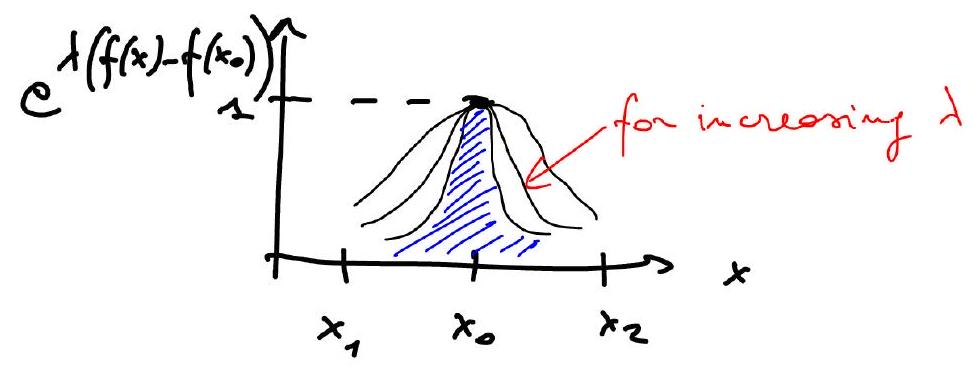
\includegraphics[max width=\textwidth, center]{2025_10_19_6d9f59a2c3b97d481c52g-1}

There one essentially three cases:

\begin{enumerate}
  \item $x_{0}$ is an interior moximum, $x_{1}<x_{0}<x_{2}$ and $f^{\prime}\left(x_{0}\right)=0$ We assume that $f^{\prime \prime}\left(x_{0}\right)<0 \quad$ (actually if $f^{\prime}\left(x_{0}\right)=f^{\prime \prime}\left(x_{0}\right)=f^{\prime \prime \prime}\left(x_{0}\right)=0$ but $f^{(i v)}\left(x_{0}\right)<0$ we con apply very similar ideas and the colculations are not more difficult). Also $g\left(x_{0}\right) \neq 0$\\
and it is finite.
\end{enumerate}

As we expect that the dominant contributions comes from the neighborhand of $x_{0}$ and $f(x)=f\left(x_{0}\right)+\frac{\left(x-x_{0}\right)^{2}}{2} f^{\prime \prime}\left(x_{0}\right) +\theta\left(\left|x-x_{0}\right|^{2}\right)$ as $x \rightarrow x_{0}$, we ortain\\
$I(\lambda) \cong \int_{x_{1}}^{\lambda_{2}} g(x) e^{\lambda\left(f\left(x_{0}\right)+\frac{\left(x-x_{0}\right)^{2}}{2} f^{\prime \prime}\left(x_{0}\right)\right)} d x \simeq g\left(x_{0}\right) e^{\lambda f\left(x_{0}\right)} \int_{\text {at lead }}^{x_{2}} e^{-\lambda \frac{\left|f^{\prime \prime}\left(x_{0}\right)\right|}{2}\left(x-x_{0}\right)^{2}} d x$

We chage vor. $S=\left(x-x_{0}\right) \sqrt{\frac{\left|f^{\prime \prime}\left(x_{0}\right)\right|}{2} \lambda}$ so\\
$I(\lambda)=g\left(x_{0}\right) e^{\lambda f\left(x_{0}\right)} \sqrt{\frac{2}{\lambda\left|f^{\prime \prime}\left(x_{0}\right)\right|}} \int^{\left(x_{2}-x_{0}\right) \sqrt{\frac{\left|f^{\prime \prime}\left(x_{0}\right)\right| \lambda}{2}}} e^{-s^{2}} d s=$

$$
\left(x_{1}-x_{0}\right) \sqrt{\frac{\left|4^{\prime \prime}\left(x_{0}\right)\right| \lambda}{2}}
$$

as $\lambda \rightarrow \infty \rightarrow \int_{-\infty}^{+\infty} e^{-s^{2}} d s=\sqrt{\pi}$\\
(22) $I(\lambda)=g\left(x_{0}\right) e^{\lambda f\left(x_{0}\right)} \sqrt{\frac{2 \pi}{\lambda\left|f^{\prime \prime}\left(x_{0}\right)\right|}} \quad \begin{aligned} & \text { as } \lambda \rightarrow+\infty \\ & \text { (leading order) }\end{aligned}$\\
one should prove that this is the bading onder (we did not).

Exercige: show that the next to basking order of $I(\lambda)$ in of. (22) is given by

$$
I(\lambda)=e^{\lambda f\left(x_{0}\right)} \sqrt{\frac{2 \pi}{\lambda\left|f^{\prime \prime}\left(x_{0}\right)\right|}}\left(g\left(x_{0}\right)+\frac{c}{\lambda}\right) \quad \text { os } \lambda \rightarrow \infty
$$

where $c$ is a comstant that depends on the derivatives of $f$ up to $4^{\text {th }}$ onder (at $\left.x=x_{0}\right)$ and an $g\left(x_{0}\right)$ and $g^{\prime}\left(x_{0}\right)$.\\
2) $x_{0}=x_{1}$ or $x_{0}=x_{2}$ ( $x_{0}$ is a flat endpoint) and $f^{\prime}\left(x_{0}\right)=0$.\\
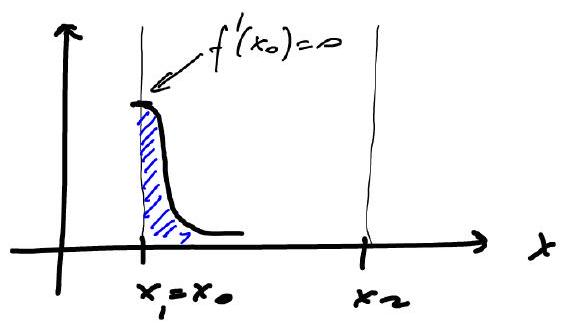
\includegraphics[max width=\textwidth, center]{2025_10_19_6d9f59a2c3b97d481c52g-3}

It is casy to show that the leading order foumbla is\\
(23)

$$
I(\lambda)=g\left(x_{0}\right) e^{\lambda f\left(x_{0}\right)} \sqrt{\frac{\pi}{2 \lambda\left|f^{\prime \prime}\left(x_{0}\right)\right|}}
$$

\section*{Example}
The modified Bessel function of second kind is a special function that occurs in mony applications. I tis given by

$$
K_{\nu}(x)=\int_{0}^{\infty} e^{-x \cosh t} \cosh (x t) d t, x>0
$$

we wish to estimate $k_{\nu}(x)$ as $x \rightarrow+\infty$ for fixed $\nu$. Since $\cosh ^{\prime}(t)=\sinh (t), t>0$, the max of $e^{-x \cosh t}$ as a function of $t(x>0)$ occurs at $t=0$, with zeno derivative.

So we con opply of (23) $\left(\cosh t \simeq 1+\frac{t^{2}}{2}+\cdots\right) f(t)=\cosh t$

$$
k_{\nu}(x)=e^{-x} \sqrt{\frac{\pi}{2 x}}
$$

as $x \rightarrow \infty$ at leading order\\
notice that it does not depend on $\nu$ !\\
Exercize: show that

$$
k_{\nu}(x)=\sqrt{\frac{\pi}{2 x}} e^{-x}\left(1+\frac{c(\nu)}{x}+\cdots\right)
$$

and $c(\nu)=\frac{4 \nu^{2}-1}{8}$.\\
3) $x_{0}=x_{1}$ or $x_{0}=x_{2}$ ( $x_{0}$ is an endpoint) but $f^{\prime}\left(x_{0}\right) \neq 0$ Without lass of generality we take $x_{0}=x_{1}$ and $f^{\prime}\left(x_{0}\right)<0$\\
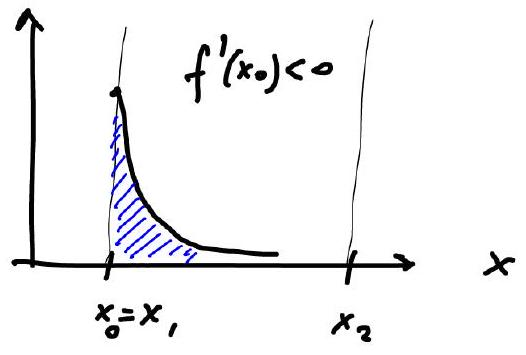
\includegraphics[max width=\textwidth, center]{2025_10_19_6d9f59a2c3b97d481c52g-4}\\
$\partial_{n}$ this cose we get $f(x)=f\left(x_{0}\right)+\left(x-x_{0}\right) f^{\prime}\left(x_{0}\right)+\cdots$\\
hence

$$
\begin{aligned}
I(\lambda) & \cong \int_{x_{1}=x_{0}}^{x_{2}} g(x) e^{\lambda\left[f\left(x_{0}\right)+\left(x-x_{0}\right) f^{\prime}\left(x_{0}\right)\right]} d x= \\
& =g\left(x_{0}\right) e^{\lambda f\left(x_{0}\right)} \int_{x_{0}}^{x_{2}} e^{\lambda\left(x-x_{0}\right) f^{\prime}\left(x_{0}\right)} d x=
\end{aligned}
$$

$$
=g\left(x_{0}\right) e^{\lambda f\left(x_{0}\right)} \int_{0}^{x_{2}-x_{0}} e^{\lambda f^{\prime}\left(x_{0}\right) s} d s=\frac{g\left(x_{0}\right) e^{\lambda f\left(x_{0}\right)}}{\lambda f^{\prime}\left(x_{0}\right)}\left[e^{\lambda s f^{\prime}\left(x_{0}\right)}\right]_{0}^{x_{2}-x_{1}}=
$$

$=\frac{g\left(x_{0}\right) e^{\lambda f\left(x_{0}\right)}}{\lambda f^{\prime}\left(x_{0}\right)}\left(e^{\lambda\left(x_{2}-x_{1}\right) f^{\prime}\left(x_{0}\right)}-1\right)$\\
as $\lambda \rightarrow \infty$ and $f^{\prime}\left(x_{0}\right)<0$ we get\\
(24)

$$
I(\lambda) \cong g\left(x_{1}\right) \frac{e^{\lambda f\left(x_{1}\right)}}{\lambda\left|f^{\prime}\left(x_{1}\right)\right|} \quad \text { as } \lambda \rightarrow \infty
$$

\section*{Example:}
Obtain the leading order approximation of

$$
I(\lambda)=\int_{0}^{1} x^{m} e^{\lambda\left(3 x^{2}+2 x^{3}\right)} d x \quad \text { as } \lambda \rightarrow+\infty
$$

\begin{center}
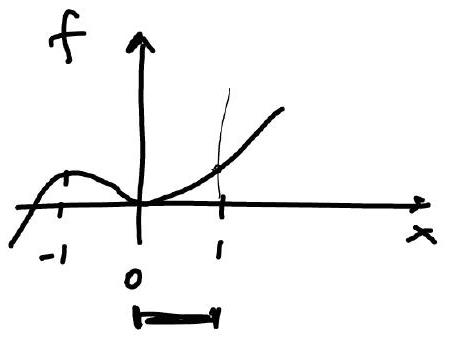
\includegraphics[max width=\textwidth]{2025_10_19_6d9f59a2c3b97d481c52g-5}
\end{center}

The max is at $x=1, f(1)=5, f^{\prime}(1)=12 g(1)=1$. We con apply ep. (24)

$$
I(\lambda) \simeq \frac{e^{5 \lambda}}{12 \lambda}
$$

\section*{Exercize:}
Calculate the leading roler approx. when the integral is

$$
\int_{-1}^{0} \cdots=? \quad \int_{-2}^{0} \cdots=?
$$

\section*{stinling formula}
We want to estimate how fast $N$ ! goes to infinits as $N \rightarrow \infty$. We will apply the Laplace's mathod to the gone me function:\\
(25)

$$
\Gamma(\lambda)=\int_{0}^{\infty} x^{\lambda-1} e^{-x} d x \quad \lambda>0
$$

Exercige: Show that $\Gamma(\lambda+1)=\lambda \Gamma(\lambda)$ hence $\lambda!=\Gamma(\lambda+1)$ which generalize the factorial to complex numbers.

Let's consider $\Gamma(\lambda+1)=\int_{0}^{a} x^{\lambda} e^{-\lambda} d x$. If we write this as $\int_{0}^{\infty} \tilde{e}^{-x} e^{\lambda h x} d x$ we comnot apply Loplace's method. It is unore beneficial to consider the mox of the function $f(x)=-x+\lambda \ln x$ and set $g(x)=1$. The mox occurs at $x=\lambda$ which sugfests a charg of vas : $x=\lambda t$ (so the max is nour fixed w.r.t. +). We get

$$
\Gamma(\lambda+1)=\int_{0}^{\infty} x^{\lambda} e^{-\lambda} d x=\lambda^{\lambda+1} \int_{0}^{\infty} t^{\lambda} e^{-\lambda t} d t
$$

$t^{\lambda} e^{-\lambda t}=e^{\lambda(\ln t-t)} \quad h(t)=\ln t-t, \quad h^{\prime}(1)=0, h^{\prime \prime}(1)=-1$, $\partial$ an this way we con apply $\varphi$. (22) with $g(t)=1 \quad\left(t_{0}=1\right)$.


\begin{equation*}
\Gamma(\lambda+1)=\lambda!\simeq \lambda^{\lambda+1} e^{-\lambda} \sqrt{\frac{2 \pi}{\lambda}} \quad \text { os } \lambda \rightarrow \infty \text {. } \tag{26}
\end{equation*}


Exercife: Show that at leading order

$$
\int_{0}^{\infty} e^{-\lambda t} e^{-\frac{1}{t}} d t \cong \frac{\sqrt{\pi} e^{-2 \sqrt{\lambda}}}{\lambda^{3 / 4}} \quad \text { as } \lambda \rightarrow \infty
$$

\section*{Example :}
Let's consider the class of ininguls:

$$
I_{m}(x)=\int_{0}^{\infty} t^{m} e^{-\frac{t^{2}}{2}-\frac{x}{t}} d t \quad x>0 .
$$

We calculate Im( $x$ ) for lagg $x$ and fixed m.\\
$\frac{t^{2}}{2}+\frac{x}{t}$ has a movable min at $\frac{d}{d t}\left(\frac{t^{2}}{2}+\frac{x}{t}\right)=0, \bar{t}=x^{1 / 3}$ So we introduce the new variable $\tau$ :

$$
t=x^{1 / 3} \tau
$$

So

$$
I_{m}(x)=x^{\frac{m+1}{3}} \int_{0}^{\infty} \tau^{m} e^{-x^{2 / 3}\left(\frac{\tau^{2}}{2}+\frac{1}{\tau}\right)} d \tau
$$

He min of the exponent occcrs at $\tau=1$ (interior) so we can apply $\varphi$. (22):

$$
\begin{aligned}
I_{m}(x) & =x^{\frac{m+1}{3}} e^{-\frac{3}{2} x^{2 / 3}} \sqrt{\frac{2 \pi}{x^{2 / 3} \cdot 3}} \\
& =x^{m / 3} e^{-\frac{3}{2} x^{2 / 3}} \sqrt{\frac{2 \pi}{3}}
\end{aligned}
$$

as $x \rightarrow \infty$.\\
leading onder, fixed $m$

Exercipes:

$$
\begin{aligned}
& \int_{-2}^{0} e^{t} e^{\lambda\left(3 t^{2}+2 t^{3}\right)} d t \simeq e^{\lambda-1} \sqrt{\frac{\pi}{3 \lambda}} \\
& \int_{0}^{1} e^{t} e^{\lambda\left(3 t^{2}+2 t^{3}\right)} d t \simeq \frac{e^{5 \lambda+1}}{12 \lambda} \\
& \int_{0}^{1} \sqrt{1+t} e^{\lambda\left(2 t-t^{2}\right)} d t \simeq e^{\lambda} \sqrt{\frac{\pi}{2 \lambda}} \\
& \int_{-1}^{2} e^{\lambda\left(t^{3}-1\right)}\left(1+t^{2}\right) d t=\frac{5 e^{6 \lambda}}{11 \lambda}
\end{aligned}
$$

Question: Let's assume that $f(x)$ behoves like in the fis:\\
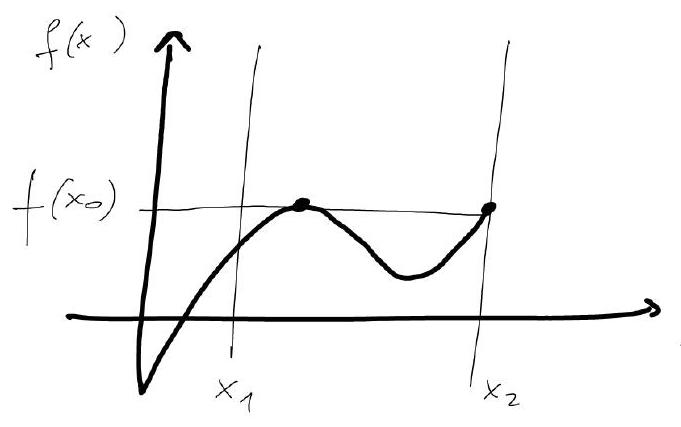
\includegraphics[max width=\textwidth, center]{2025_10_19_6d9f59a2c3b97d481c52g-8}

Where does the leading onder come from?


\end{document}